%===============================================================================
% $Id: ifacconf.tex 19 2011-10-27 09:32:13Z jpuente $  
% Template for IFAC meeting papers
% Copyright (c) 2007-2008 International Federation of Automatic Control
%===============================================================================
\documentclass{ifacconf}



\usepackage{graphicx}      % include this line if your document contains figures
\usepackage{natbib}        % required for bibliography
\usepackage{epsfig}
\usepackage{amsmath}
\usepackage{amssymb}
\usepackage{mathrsfs}

\usepackage{todonotes}
\newcommand{\NOTE}[1]{\todo[inline]{#1}}

\newcommand*{\Resize}[1]{\resizebox{\columnwidth}{!}{$#1$}}

\DeclareMathAlphabet{\mathpzc}{OT1}{pzc}{m}{it}

\providecommand{\norm}[1]{\left\|#1\right\|}
\providecommand{\abs}[1]{\left|#1\right|}
\providecommand{\conv}{\text{conv}}

\usepackage{xcolor}
\def\edit{\textcolor{blue}}
\allowdisplaybreaks[4]


%===============================================================================
\begin{document}
\begin{frontmatter}

% predefined environments
%\begin{thm} ... \end{thm}		% Theorem
%\begin{lem} ... \end{lem}		% Lemma
%\begin{claim} ... \end{claim}	% Claim
%\begin{conj} ... \end{conj}	% Conjecture
%\begin{cor} ... \end{cor}		% Corollary
%\begin{fact} ... \end{fact}	% Fact
%\begin{hypo} ... \end{hypo}	% Hypothesis
%\begin{prop} ... \end{prop}	% Proposition
%\begin{crit} ... \end{crit}	% Criterion
%\begin{rem} ... \end{rem}    % Remark
%\begin{pf} ... \end{pf}      % Proof
%\begin{ack} ... end{ack}     % Acknowledgement

\title{Robust receding horizon control for linear systems with state dependent disturbance} 


\thanks[footnoteinfo]{Supported by the Martin Senior Scholarship of Worcester College, Oxford.}

\author[Oxford]{Rainer M. Schaich\thanksref{footnoteinfo}} 
\author[Oxford]{Mark Cannon} 

\address[Oxford]{Department of Engineering Science, University of Oxford, OX1 3PJ, UK. (e-mail: 
rainer.schaich@eng.ox.ac.uk, mark.cannon@eng.ox.ac.uk).}

\begin{abstract}                % Abstract of not more than 250 words.

\end{abstract}

\begin{keyword}
-
\end{keyword}

\end{frontmatter}
%===============================================================================

\section{Introduction}\label{sec:intro}

Robust model predictive control (RMPC) algorithms compute a control law that optimises a predicted performance
criterion subject to state and control constraints for all possible realisations of model
uncertainty. \citet{Witsenhausen:1968} proposes to formulate the RMPC problem as a game in which the adversary
tries to maximise the effect of model uncertainty on the cost and the controller chooses its strategy to
minimise the cost for the worst case system parameters and disturbances. This formulation is widely accepted
in the RMPC literature \citep[e.g.][]{Bemporad:1999,Bemporad:2003,Lee:1997}.
%see e.g.~\cite{Bemporad:1999,Bemporad:2003,Lee:1997}.  
The predicted control law may be an open-loop policy, in which case the controller chooses its strategy for
the whole prediction horizon before the adversary decides its strategy, or a closed-loop policy in which the
horizon is split into stages and the actions of controller and adversary at each stage depend on the
outcome of the previous stage). Theoretical properties of these controllers are well understood \citep[e.g.][]{Mayne:2000}. However, the numerical computation of robust model predictive controllers still poses
a challenge and only few tractable solutions have been proposed.

Various strategies have been proposed to solve RMPC problems for linear systems subject to linear state and
input constraints, with model uncertainty in the form of bounded additive disturbances and/or multiplicative
parameters. For the case of unknown additive disturbances, \citet{Scokaert:1998} propose a scenario-based
approach to solve a sequence of min-max problems online, however the computational complexity of this approach
grows exponentially with the length of the horizon. A parametrised algorithm was proposed
by~\cite{Rakovic:2012} which reduces the RMPC problem to a single linear program to be solved online, but
although this is a closed loop strategy the parametrisation is in general suboptimal. Explicit RMPC algorithms
optimise the worst case predicted performance for each admissible model state offline and
%exploit the structure of the solution using results
use results from multi-parametric programming to parametrise the optimal control law as a piecewise affine function of the
state \citep[e.g.][]{Bemporad:2003,Diehl:2004}. However, this requires extensive offline computation and
becomes inefficient for a high-dimensional state space.
An alternative approach that similarly exploits the piecewise affine structure of the solution, but with
less redundancy, was proposed by~\cite{Buerger:2011} and extended in~\cite{Buerger:ACC}. In this work an active set
solver is designed to solve a sequence of min-max problems explicitly online. 

In all of this work and, to the authors' best knowledge, in all of the published literature on algorithmic
solutions to the RMPC problem, the disturbances are confined to sets that are assumed to be constant,
i.e.~independent of the system state and control inputs. Recent algorithmic advances~\citep{Schaich:2015}
make it possible to treat polytopic disturbance sets that depend in an affine manner on the system state and the control
input. This provides an algorithmic and analytical framework which is used in the
current paper to embed affine state and input dependent disturbance constraints into the framework of the
active set RMPC solver framework proposed by~\cite{Buerger:2011}. Disturbances that belong to sets which depend
on model states and inputs can account for multiplicative model uncertainty as well as linearisation
errors, and the approach of this paper is therefore able to handle linearisation errors in RMPC non-conservatively.
%, as will be shown in an example.

After describing the control problem in Section~\ref{sec:problem:statement} we summarise preliminary 
results which are necessary to formulate the considered problem explicitly (Section~\ref{sec:preliminaries}).
Section~\ref{sec:gen:mpQP} discusses the recursive solution for equality constrained min-max recursions, one of 
the essential parts of the active set solver, and this is applied to the min-max RMPC problem in Section~\ref{sec:applied:mpQP}
for the case that the active set of constraints is known. A line search to determine the active set of constraints is presented
in Section~\ref{sec:line:search}. The application of the proposed algorithm to an example problem is presented in 
Section~\ref{sec:example} and conclusions are drawn in Section~\ref{sec:conclusion}.



\section{Problem Statement}\label{sec:problem:statement}
We consider a computationally efficient method for solving online min-max receding horizon control problems
that exploits the structure of multi-parametric programming solutions. Our approach determines the optimal
feedback law without approximating the cost or the constraints of the problem, and without making restrictive
assumptions on the parametrisation of control inputs.
%This broadens the applicability of the approach, allowing for higher order models and longer
%prediction horizons than 
%
%The high computational complexity of online min-max receding horizon control schemes generally requires either
%that the solution is approximated or that their application is limited to problems involving simple system models and short horizons. Here we consider an
%efficient method for solving min-max problems that exploits the structure of multi-parametric programming
%solutions.
%The set of systems to which a min-max robust receding horizon control scheme can be applied online 
%without approximating the solution is bounded by the system complexity. The way to solve min-max problems we 
%adopt here, is to use the structure of the solution to derive multi-parametric programs that can be solved
%efficiently. In order to be able to obtain a closed form solution of the min-max program simple optimisation
%formulations have to be
%The algorithmic treatment of min-max problems
%involving state constraints and disturbances constrained to lie in fixed polytopic disturbance sets was
%introduced in~\cite{Bertsekas:1971}. Recently~\cite{Schaich:2015} proposed an algorithm to compute the so called maximal
%robust positive invariant (MRPI) sets (see~\cite{blanchini:2007}) for linear systems subject to state and
%input dependent disturbance constraints. In this paper we develop the algorithm further
%to compute polytopic constraints necessary to satisfy state constraints robustly in this setup. We
%present a robust receding horizon control scheme for
%
To make it possible to obtain a closed form solution of the min-max optimal control problem we assume a
linear-quadratic problem formulation. Thus we assume the linear dynamic model 
\begin{equation}\label{eq:system:equation}
	x^+ = A x + B u + D w,
\end{equation}
%
where $A,B,D$ are real matrices of appropriate dimension, $x,  x^+\in\mathcal X\subseteq\mathbb R^n$ denote the state 
and successor state respectively, $u\in\mathcal U=\{u:Fu\leq{\bf{1}}\}\subset\mathbb R^p$ is the control input
and $w\in\mathcal W(x,u)\subset\mathbb R^q$ is an unknown disturbance input. The disturbance set $\mathcal
W(x,u)$ is assumed to have a known dependence on the values of $x$ and $u$, according to
%
\begin{equation}\label{eq:PWA:def:disturbance}
	\mathcal W(x,u) = \{w: Gw \leq H(x,u)\},
\end{equation}
%
where $H(x,u)$ is an elementwise convex, piecewise affine function. The control objective is to minimize the
worst case value, over all future model uncertainty, of the cost
\begin{equation}\label{eq:quadratic:cost}
\sum_{k=0}^\infty \bigl( \|x_k\|_Q^2 + \|u_k\|_R^2 - \gamma^2 \|w_k\|^2 \bigr) ,
\end{equation}
where the subscript $k$ denotes the realisation of a variable at time $k$, $\|x\|_Q^2$ denotes the quadratic
form $x^TQx$, $Q$ and $R$ are given positive definite
matrices and $\gamma$ is a given scalar weight that controls the $l^2$-gain of the closed loop system from the
disturbance sequence to the state and control sequences.

Given a prediction horizon of $N$ steps over which the predicted control law is to be optimized, we define the
min-max optimal control problem with $m$ stages to go as
%
\begin{subequations}\label{eq:the:problem}%
\begin{equation}
	J_{m}^\ast(x) = \min_u \max_{w,x^+} \tfrac{1}{2}\bigl(\norm{x}_Q^2+\norm{u}_R^2-\gamma^2
    \norm{w}^2\bigr) + J_{m-1}^\ast(x^+)
\end{equation}
subject to
\begin{gather}
	x^+ = A x + B u + D w\\
	u\in\mathcal U \\
	w\in\mathcal W(x,u) \\
	(x,u)\in\mathcal Z_m
\end{gather}
\end{subequations}
%
for $m=1,\ldots,N$, with $J_0^\ast(x) = \|x\|_{P_0}^2$.
The stagewise  state and input constraints $\mathcal Z_m$ are defined recursively by
%
\begin{subequations}\label{eq:definition:stage:constraints}
\begin{align}
	\mathcal Z_m &= \{(x,u)\,: u\in\mathcal U \nonumber\\
	&\quad\ \wedge \; A x + Bu + Dw\in\mathcal X_{m-1}\; \forall\, w\in\mathcal W(x,u)\} 
	\label{eq:definition:mixed:stage:constraint}\\
	\mathcal X_m &= \{x : \exists\, u\in\mathcal U, (x,u)\in\mathcal Z_m\}
	\label{eq:definition:state:stage:constraint}\\
\end{align}
with
\begin{equation}
	\mathcal X_0 = \mathcal X^\infty .
\end{equation}
\end{subequations}
Thus the constraints $(x,u)\in\mathcal Z_m$ ensure that the terminal state, namely $x^+$ at $m=1$, is
contained in $\mathcal{X}^\infty$. We define $\mathcal{X}^\infty$ as the maximal robust positive invariant (MRPI) set \citep{blanchini:2007}), for the closed-loop system governed by a fixed state feedback controller
$u=Kx$, so that 
%
\begin{equation}\label{eq:definition:MRPI:set}
	\mathcal X^\infty = \{x: (A+BK)x + Dw \in \mathcal X^\infty \forall w\in\mathcal W(x,Kx)\},
\end{equation}
%
and we define $P_0$ so that $J_0^\ast(x)$ is the worst case value of the cost (\ref{eq:quadratic:cost}) under
$u=Kx$ in the absence of constraints.
Recently~\cite{Schaich:2015} proposed an algorithm to compute MRPI sets
for linear systems subject to state and input dependent disturbance constraints. In this paper we combine this approach
with the multistage multi-parametric programming method of~\cite{Buerger:ACC} to derive an efficient algorithmic
solution to the online MPC optimization of (\ref{eq:the:problem}a-e).



\section{Controllable sets}\label{sec:preliminaries}
In this section we summarise results on controllable sets that allow the constraints of the problem~\eqref{eq:the:problem} to be to formulated
in a convenient way. The following result shows that the MRPI set (\ref{eq:definition:MRPI:set}) associated
with the pointwise polytopic set~\eqref{eq:PWA:def:disturbance} is polytopic if $H$ is elementwise convex and
piecewise affine. For a proof and detailed discussion of this result we refer the reader
to~\cite{Schaich:2015}.
%
\begin{lem}\label{thm:MRPI:set:is:polytopic}
Let $\mathcal X \subseteq \{x:\Gamma x\leq{\bf{1}}\wedge-\Gamma x\leq{\bf{1}}\}$ be polyhedral, and the pair $(A+BK,\Gamma)$ be
observable, furthermore let $\mathcal W(x,Kx)$ be defined as in~\eqref{eq:PWA:def:disturbance} with a elementwise convex piecewise
affine function $H(x,Kx)$ which is bounded for all finite $x$. Then the MRPI set $\mathcal X^\infty$ is a polytope, i.e.
it has the representation 
\begin{equation}\label{eq:halfspace:representation:MRPI}
	\mathcal X^\infty=\{x:\Lambda_i x\leq \lambda_i, \forall\, i\in\mathcal I^\infty\}.
\end{equation}
\end{lem}
%
We need to emphasise the following 
\begin{rem}\label{rem:vertex:representation}
Note that an essential assumption in Lemma~\ref{thm:MRPI:set:is:polytopic} is that $\mathcal W(x,u)$ is a polytope
for all finite $(x,u)$, i.e. it has a convex hull representation $\mathcal W(x,u) = \conv_k\{w_k(x,u)\}, k\in\{1,\dots,r\}$ where each 
vertex, $w_k(x,u)$, is a piecewise affine function of $(x,u)$, i.e.
\begin{multline}
	w_k(x,u) = \max\{W_{k,1}^x x + W_{k,1}^u u + w_{k,1}, \\
        W_{k,2}^x x + W_{k,2}^u u + w_{k,2},\dots\}
\end{multline}
where the maximisation is performed elementwise.
\end{rem}
%
We now derive the representation of $\mathcal Z_m$ and $\mathcal X_m$ as defined in~\eqref{eq:definition:stage:constraints}.
According to Lemma~\ref{thm:MRPI:set:is:polytopic} the MRPI set $\mathcal X^\infty$ is polytopic and has the 
representation~\eqref{eq:halfspace:representation:MRPI}. Therefore the recursion~\eqref{eq:definition:mixed:stage:constraint}
defines $\mathcal Z_1$ as
\begin{equation}\label{eq:derivation:of:mpLP:stage:constraints}
\begin{aligned}
	\mathcal Z_1 =& (\mathbb R^n\times\mathcal U)\cap 
\begin{aligned}[t] \Bigl\{(x,u): \Lambda_{0,i}(Ax&+Bu+Dw)\leq \lambda_{0,i} \\
& \forall w\in\mathcal W(x,u),\, i\in\mathcal I_0 \Bigr\} \end{aligned}
\\
	=&\begin{aligned}[t] (\mathbb R^n & \times \mathcal U) \cap\Bigl\{ (x,u): \\
& \max_{w\in\mathcal W(x,u)}\Lambda_{0,i}(Ax+Bu+Dw)\leq\lambda_{0,i},\, \forall i\in\mathcal I_0 \Bigr\} \end{aligned}
\\
	=&\begin{aligned}[t] & (\mathbb R^n \times\mathcal U)\cap \Bigl\{ (x,u): \\
& \!\!\!\!\!\!
\Lambda_{0,i}(Ax+Bu)+ \!\!\underbrace{\max_{j\in\{1,\dots,r\}}\Lambda_{0,i} Dw_j(x,u)}_{(i)}\leq\lambda_i, \, \forall i\in\mathcal I_0
	\Bigr\} \end{aligned}
\end{aligned}
\end{equation}
Since the maximisation $(i)$ in \eqref{eq:derivation:of:mpLP:stage:constraints} is a multi-parametric
linear program, its solution is piecewise affine in $(x,u)$. 
Therefore the set $\mathcal Z_1$ has a representation
$\mathcal Z_1=\{(x,u):\Xi^x_{1,i}x+\Xi^u_{1,i}u\leq\xi_{1,i},i\in\mathcal J_1\}$. The projection~$\mathcal X_1$ 
of $\mathcal Z_1$ onto~$\mathbb R^n$ is therefore has the representation~$\mathcal X_1 = \{x:\Lambda_{1,i} x\leq\lambda_{1,i},i\in\mathcal I_1\}$.
From here the determination of $\mathcal Z_k$ and $\mathcal X_k$ follows recursively. We are now able to formulate 
all constraints in~\eqref{eq:the:problem} as inequalities. In the next section we discuss a method of solving
min-max programs such as~\eqref{eq:the:problem} efficiently.


\section{Solving equality constrained multi-parametric quadratic programs}\label{sec:gen:mpQP}
In this section we discuss equality constraint multi-parametric quadratic programs (mpQP) 
(see~\cite{bemporad02,Tondel:2003} for an extended discussion), as they are essential in the treatment 
of the considered min-max program using an active set solver. 
%Note that the notation in this section does not refer to the notation in the preceding and proceeding sections.
Consider the primal equality-constrained concave mpQP
\begin{equation}\label{mpQP:primal}
	V(\theta) = \left\{\begin{split}
	\max_{y} & \;\frac{1}{2} y^T W y + c^Ty + d\\
	\text{s.t.} &\; Hy  = f +S\theta
	\end{split}\right.
\end{equation}
%where  $y\in\mathbb{R}^{n_y}$ is the optimization variable, 
where $W\preceq 0$, $c$, $d$, $H$, $f$, $S$ are constants and $\theta$ is a variable parameter. We wish to
know how the solution of (\ref{mpQP:primal}) varies with $\theta$.  The Lagrangian function
associated with~\eqref{mpQP:primal} is
\[
	L(y,\lambda,\theta)  = \frac{1}{2} y^T W y + c^Ty + d + \lambda^T(Hy - f - S\theta)
\]
and the dual problem is the unconstrained mpQP
\begin{equation}\label{mpQP:dual}\begin{split}
	\min_\lambda &\; \mathcal D(\lambda,\theta)= \min_\lambda-\frac{1}{2}\lambda^T H W^{-1}H^T \lambda 
	-(HW^{-1}c\\ &+ f + S\theta)^T\lambda
	-\frac{1}{2}c^TW^{-1}c +d
\end{split}\end{equation}
To solve~\eqref{mpQP:primal} we consider the first order optimality conditions, see e.g.~\cite{Fletcher:2000}:
\begin{equation}\label{kkt:conditions}
	\begin{aligned}
        W y + H^T\lambda & = -c \\
        H y &= f + S\theta.
	\end{aligned}
\end{equation}

\begin{lem}\label{lem:mpQP:solution}
The solution of~\eqref{kkt:conditions} has the representation
\begin{equation}\label{mpQP:solution}
	\begin{split}
		y &= M_\theta \theta + m\\
		\lambda &= N_\theta \theta + N_\beta \beta + n
	\end{split}
\end{equation}
where $N_\beta\neq 0$ only if $H$ is not right invertible, in which case $H^TN_\beta=0$ and the columns
of $N_\beta$ span ker$(H^T)$.
\end{lem}
%
The matrices $M_\theta$, $N_\theta$, $N_\beta$ and vectors $m$, $n$
are constant and the variable $\beta$ is used to parametrise the solution in the null space
of~\eqref{kkt:conditions}. We say (\ref{mpQP:primal}) is \textit{degenerate} if $N_\beta\neq 0$.
%
\begin{pf}
If $H$ is not right invertible, then we must have rank$(H)=n_y<n_\lambda$ or
rank$(H)<\min\{n_y,n_\lambda\}$.
For the case that rank$(H)=n_y$ (i.e.\ $H$ has full rank and $n_y<n_\lambda$), 
using the QR-decomposition \citep[e.g.][]{Nocedal:2006} of $H=(Q_1,Q_2)\cdot(R^T,0)^T$ the solution 
is given by $(m^T,n^T)^T = \Sigma (-c^T,f^T)^T$, $(M_\theta^T,N_\theta^T)^T = 
\Sigma (0,S^T)^T$ and $N_\beta=Q_2$, where 
\[
	\Sigma = \left(\begin{array}{cc}
	0 & R^{-1}Q_1^T \\
	Q_1 R^{-T} & -Q_1R^{-T}WR^{-1}Q_1^T
	\end{array}\right) .
\]
On the other hand if rank$(H)<\min\{n_y,n_\lambda\}$ (so that $H$ is rank deficient), then
\[
	\Sigma = \left(\begin{array}{cc}
	W^{-1}-W^{-1}R^T\Delta RW^{-1} & W^{-1}R^{T}\Delta Q_1^{T}\\
	Q_1\Delta R W^{-1} & -Q_1\Delta Q_1^T
	\end{array}\right)
\]
with $\Delta = (RW^{-1}R^T)^{-1}$. This concludes the proof.
\end{pf}
%
Since the degeneracy variable $\beta$ does not appear in the
primal optimiser, it does not affect the primal objective value of~\eqref{mpQP:primal}.
However, substituting~\eqref{mpQP:solution} into the dual objective~\eqref{mpQP:dual} yields
\begin{align*}
\mathcal D(&\lambda(\theta,\beta),\theta) = \\
& {-\tfrac{1}{2}}(N_\theta \theta + N_\beta \beta + n)^T H W^{-1}H^T 
	(N_\theta \theta + N_\beta \beta + n)\\
& -(AW^{-1}c + 
	f + S\theta)^T(N_\theta \theta + N_\beta \beta + n) -\tfrac{1}{2}c^TW^{-1}c,
\end{align*}
which is unbounded if
\[
	(f^T+\theta^TS^T)N_\beta \neq 0
\]
and can be made arbitrarily small by the choice of $\beta$. Therefore we restrict $\theta$ to satisfy 
\begin{equation}\label{mpQP:compatability:assumption}
	N_\beta^Tf = -N_\beta^TS\theta,
\end{equation} 
so that the dual mpQP has a unique solution
and the choice of $\beta$ does not affect either the primal or the dual cost and can be used for
any purpose. For a general mpQP, condition~\eqref{mpQP:compatability:assumption} is a restriction on the set
of parameters for which~\eqref{mpQP:primal} has a solution of the form~\eqref{mpQP:solution}.
In our multi-stage min-max setup, the parameter is the optimiser of a subsequent optimisation
problem and can be ensured to satisfy~\eqref{mpQP:compatability:assumption} by the so called 
compatibility constraint. The optimal objective of~\eqref{mpQP:primal} is given by
\begin{equation}\label{mpQP:cost:to:go}\begin{split}
	V(\theta) = &\frac{1}{2}\theta^T M_\theta^T W M_\theta \theta + c^TM_\theta \theta \\
& + m^TWM_\theta+\frac{1}{2}m^T Wm + c^Tm\\
=&\frac{1}{2} \theta^T W_\theta \theta + c^T_\theta \theta + d_\theta.
\end{split}\end{equation}
%
Suppose now that we want to solve a problem that depends on the solution of~\eqref{mpQP:primal} and an
additional parameter $\phi$:
\begin{equation}\label{mpQP:second:stage} 
	J(\phi) = \left\{\begin{array}{rl}
	\min_\theta & \frac{1}{2}\theta^T\Phi\theta + g^T\theta + f + V(\theta)\\
	\text{s.t.} & C\theta = e+T\phi
	\end{array}\right.
\end{equation}
where $\Phi$, $C$, $g$, $f$, $C$, $e$, $T$ are constants and
the equality constraints include~\eqref{mpQP:compatability:assumption}. Since we know
that the optimal cost-to-go $V(\theta)$ has the structure~\eqref{mpQP:cost:to:go},
the problem~\eqref{mpQP:second:stage} reduces to a problem with the form of~\eqref{mpQP:primal},
which yields a solution similar to~\eqref{mpQP:solution}, i.e.
\begin{equation}
\begin{split}
	\theta &= K_\phi \phi + k\\
	\eta &= L_\phi \phi + L_{\hat\beta} \hat\beta + l
\end{split}
\end{equation}
where $\eta$ is the dual variable, and $\Phi+W_\theta\succ 0$ has been assumed. Finally we note 
that~\eqref{mpQP:compatability:assumption} is only nontrivial if~$H$ is not right invertible and only 
introduces as many constraints on~$\theta$ as there are linearly
dependent rows in~$H$.

In the solution of recursive min-max programs such as~\eqref{eq:the:problem} we use the composition of
the stage optimisers, i.e. we use $y(\theta(\phi)) = M_\theta K_\phi \phi + (M_\theta k + m)$.
Notice that this composition of optimisers is again an affine function of the parameter $\phi$, in particular
we will exploit the fact that parameter variations along lines translate to lines in the optimiser
space as long as no activations or deactivations of constraints occur. We will revisit this fact
when we perform a line search in order to update the active constraints.


\section{Solving min-max quadratic programs as multi-parametric quadratic programs}\label{sec:applied:mpQP}
In this section we apply the results derived in section~\ref{sec:gen:mpQP} to
the considered min-max robust control problem~\eqref{eq:the:problem}. We 
define a recursion and assume the active set is known to obtain a closed solution for~\eqref{eq:the:problem}.
%
%To use an active set solver for the problem:
First epx
\begin{subequations}\label{eq:the:problem:reformulated}%
\begin{equation}
	J_{m}^\ast(x) = \min_u \max_{w,x^+} \tfrac{1}{2}\bigl(\norm{x}_Q^2+\norm{u}_R^2-\gamma^2
    \norm{w}^2\bigr) + J_{m-1}^\ast(x^+)
\end{equation}
subject to
\begin{gather}
	x^+ = A x + B u + D w
\\
\label{eq:dist:cons}
	G w \leq  H(x,u)
\\
\label{eq:state:constraints}
	\Xi^x_m x + \Xi^u_m u \leq \xi_m
\\
	\hat C_m x^+ = - {\bf{1}}
\\
	C_m^x x + C_m^u u  = {\bf{1}}
\end{gather}
\end{subequations}
with~$J_0^\ast(x^+) = \frac{1}{2}\norm{x^+}_P^2$ and $m=1,\dots,N$. Notice that explicitly using
$u\in\mathcal U$ is no longer necessary as satisfaction of the input constraints is intrinsic
if $(\cdot,u)\in\mathcal Z_m$.
We split the sequence of  min-max problems into a sequence of multi-parametric 
quadratic programs. Starting with the maximisation at stage $m=1$ and using a backward sweep approach (see e.g.~\cite{Bryson:1975}), 
we obtain
\begin{equation}
	\hat J_m^\ast(x,u) = \left\{\begin{split}
    \max_{w,x^+} & -\frac{\gamma^2}{2}\norm{w}^2 + J_{m-1}^\ast(x^+)\\
    \text{s.t.} & \begin{array}{rcl}
    Gw & \leq & H(x,u)\\
    x^+ & = & Ax + Bu + Dw\\
    \hat C_m x^+ &=& -{\bf{1}}
    \end{array}
    \end{split}\right.
\end{equation}
and
\begin{equation}
	J_m^\ast(x) = \left\{\begin{split}
    \min_{u} & \frac{1}{2}\left(\norm{x}^2_Q + \norm{u}_R^2\right) + \hat J_m^\ast(x,u)\\
    \text{s.t.} & \begin{array}{ccccl}
    \Xi^x_m x &+& \Xi^u_m u &\leq &\xi_m\\
    C_m^x x &+ & C^u_m u & = & {\bf{1}}
    \end{array}
    \end{split}
    \right.
\end{equation}
Suppose the active set is given, i.e.~it is known which inequality constraints hold with equality. 
For notational convenience we denote active inequalities with $(\cdot)^\prime$, e.g.  $(\Xi^x_m)^\prime x + (\Xi^u_m)^\prime u = \xi_m^\prime$. 
Since $J^\ast_0(x^+) = \frac{1}{2}\norm{x^+}_{P_0}^2$ is a given function, compatibility constraints are not necessary at 
stage $m=1$ and the maximisation problem is given by:
\begin{equation}
	\hat J_1^\ast(x,u) = \left\{\begin{split}
	\max_{w,x^+} & -\frac{\gamma^2}{2}\norm{w}^2 + J_{0}^\ast(x^+)\\
	\text{s.t.} & 
	\underbrace{\left(\begin{array}{cc}
	G^\prime & 0 \\ -D & I
	\end{array}\right)}_{\bar H}
	\left(\begin{array}{c}w\\ x^+\end{array}\right)
	\\&= \underbrace{\left(\begin{array}{cc}W_x^\prime & W_u^\prime \\ A & B\end{array}\right)}_{
	\bar S
	}
	\left(\begin{array}{c}x \\ u \end{array}\right) + \underbrace{\left(\begin{array}{c}
	w_c^\prime \\ 0\end{array}\right)}_{\bar f}
	\end{split}\right.
\end{equation}
with $W_x^\prime, W_u^\prime$ and $w_c^\prime$ denoting the active rows of the right hand side 
of~\eqref{eq:dist:cons}.
With Lemma~\ref{lem:mpQP:solution} we obtain
\begin{equation}
      \left(\begin{array}{c}
      w^\ast \\
      x^{+,\ast} \\
      \eta^\ast \\
      \lambda^\ast
      \end{array}\right) = \left(\begin{array}{c}M^w_z\\ M^{x^+}_z \\ N^{\eta}_z \\ N^{\lambda}_z
      \end{array}\right)\underbrace{\left(\begin{array}{c}x\\ u\end{array}\right)}_z + 
      \left(\begin{array}{c}0\\ 0 \\ N^{\eta}_{\hat\beta} \\ N^{\lambda}_{\hat\beta}
      \end{array}\right)\hat\beta + \left(\begin{array}{c}m^w\\ m^{x^+} \\ n^{\eta} \\ n^{\lambda}
      \end{array}\right)
\end{equation}
where $\eta^\ast$ denotes the dual variable to the active inequality constraints and hence must
be non-negative, i.e.~$\eta^\ast\geq0$. Notice that we omitted stage indices to avoid overloaded notation.
The cost-to-go for the minimisation problem at stage $m=1$ is
\begin{equation}
	\hat J_1^\ast(z) = \frac{1}{2}z^T
    \hat Q_1 z + c_1 z + d_1
\end{equation}
and the compatibility constraint is given by
\begin{equation}\label{prototype:compatibility:conditions}
	N_{\hat\beta}^T(\bar S z + \bar f) = 0,
\end{equation}
i.e.\ $C_1^x$ and $C_1^u$ are given as a row wise normalised version of~\eqref{prototype:compatibility:conditions}.
Hence the minimisation problem at $m=1$ becomes
\begin{equation}
	J_1^\ast(x) = \left\{\begin{split}
	\min_{u} & \frac{1}{2}\left(\norm{x}^2_Q + \norm{u}_R^2\right) + \hat J_{1}^\ast(x,u)\\
    \text{s.t.} & 
    \underbrace{\left(\begin{array}{c}
    (\Xi_1^u)^\prime \\ C_1^u
    \end{array}\right)}_{\bar C}
    u
    = \underbrace{\left(\begin{array}{c}-(\Xi^x_1)^\prime \\ -C_1^x\end{array}\right)}_{
    \bar T
    }x + 
    \underbrace{\left(\begin{array}{c}\xi_1^\prime\\  {\bf{1}} \end{array}\right)}_{\bar e}
    \end{split}\right.
\end{equation}
and its solution is given by
\begin{equation}
	\left(\begin{array}{c}
	u^\ast \\
	\nu^\ast \\
	\hat\zeta^\ast
	\end{array}\right) = \left(\begin{array}{c}K^u_x\\ O^{\nu}_x \\ O^{\hat\zeta}_x
	\end{array}\right)x + 
	\left(\begin{array}{c}0\\ O^{\nu}_\beta \\ O^{\hat\zeta}_{\beta}
	\end{array}\right)\beta + \left(\begin{array}{c}k^u\\ o^{\nu} \\ o^{\hat\zeta}
	\end{array}\right).
\end{equation}
Here $\hat C_2$ is a normalised version of $O^T_\beta(\bar T x + \bar e) = 0$.
For completeness, the $m=2$ maximisation and its solution are:
\begin{equation}
	\hat J_2^\ast(x,u) = \left\{\begin{split}
	\max_{w,x^+} & -\frac{\gamma^2}{2}\norm{w}^2 + J_{1}^\ast(x^+)\\
	\text{s.t.} & 
	\underbrace{\left(\begin{array}{cc}
	G^\prime & 0 \\ -D & I \\
	0 & \hat C_2
	\end{array}\right)}_{\bar A}
	\left(\begin{array}{c}w\\ x^+\end{array}\right)
	\\&= \underbrace{\left(\begin{array}{cc}W_x^\prime & W_u^\prime \\ A & B \\ 0 & 0\end{array}\right)}_{
	\bar S
	}
	\left(\begin{array}{c}x \\ u \end{array}\right) + \underbrace{\left(\begin{array}{c}
	w_c^\prime \\ 0 \\ {\bf{1}}\end{array}\right)}_{\bar b}
	\end{split}\right.
\end{equation}
\begin{equation}
	\left(\begin{array}{c}
	w^\ast \\
	x^{+,\ast} \\
	\eta^\ast \\
	\lambda^\ast\\
	\zeta^\ast
	\end{array}\right) = \left(\begin{array}{c}M^w_z\\ M^{x^+}_z \\ N^{\eta}_z \\ N^{\lambda}_z \\ N^{\zeta}_z
	\end{array}\right)z + 
	\left(\begin{array}{c}0\\ 0 \\ N^{\eta}_{\hat\beta} \\ N^{\lambda}_{\hat\beta} \\ N^\zeta_{\hat\beta}
	\end{array}\right)\hat\beta + \left(\begin{array}{c}m^w\\ m^{x^+} \\ n^{\eta} \\ n^{\lambda}\\ n^\zeta
	\end{array}\right)
\end{equation}
All subsequent minimisations and maximisations can be solved analogously provided the active set is
known.


\section{Exact solution of min-max program}\label{sec:line:search}
In the previous section we presented a recursive algorithm to solve~\eqref{eq:the:problem}
when all active constraints are known. In this section we present a method to find the active
constraints for a given initial state $\mathpzc x_e$ using a line search starting from a state $\mathpzc x_0$
for which the active constraints are known. In section~\ref{sec:gen:mpQP} and~\ref{sec:applied:mpQP}
we derived an explicit solution for each sub-optimisation program which depended affinely on the
state~$x$ at that stage~$m$ or the state and the input at that stage. Henceforth we denote the stage 
with an index, e.g.~$x_m$ denotes the optimised state in stage $m$, that is $x^{+,\ast}$ at stage $m+1$.
To ensure continuity of the dual variables we choose $\hat\zeta_m = \hat\beta_m$ and $\zeta_m=\beta_{m-1}$.
The affine character of the solution of each sub-problem allows us to parametrise the entire trajectory
with respect to parameters at stage~$m=N$, that is $x_N=\chi_0$ $x_N=\mathpzc x_0$ and $\beta_N$.

We recursively define all primal and dual variables:
\begin{equation}\label{eq:trajectory:affine:representation}
	\begin{split}
		u_N(x_N) =& \underbrace{K_{x,N}^x}_{\Psi_N^u} x_N + \underbrace{k_N^u}_{\psi_N^u}\\
		\nu_N(x_N,\beta_N) &= \underbrace{O_{x,N}^x}_{\Psi_N^\nu} x_N + \underbrace{O_{\beta,N}^\nu}_{\Phi_N^\nu} \beta_N + 
		\underbrace{o_N^\nu}_{\psi_N^u}\\
		&\vdots \\
		x_0(x_N) =& \underbrace{M_{z,1}^{x^+}\left(\begin{array}{c} \Psi_2^x \\ \Psi_1^u \end{array}\right)}_{\Psi_1^x}x_N + 
		M_{z,1}^{x^+}\left(\begin{array}{c} \psi_2^x \\ \psi_1^u \end{array}\right) + m_1^{x^+}\\
		\eta_1(x_N,\beta_N) =& \underbrace{\left(N_{z,1}^{\eta}\left(\begin{array}{c} \Psi_2^x \\ \Psi_1^u \end{array}\right) + 
		N_{\hat\beta,1}^\eta \Psi_1^{\hat\zeta}\right)}_{\Psi_1^\eta}x_N + \underbrace{N_{\hat\beta,1}^\eta \Phi_1^{\hat\zeta}}_{\Phi_1^\eta} \beta_N\\
		&+\underbrace{N_{z,1}^{\eta}\left(\begin{array}{c} \psi_2^x \\ \psi_1^u \end{array}\right) + 
		N_{\hat\beta,1}^\eta \psi_1^{\hat\zeta} + n_1^\eta}_{\psi_1^\eta}\\
		&\vdots
	\end{split}
\end{equation}
Notice that $\Phi^{(\cdot)}_m$ is only non-trivial if the associated sub-problem is degenerate. The 
representation~\eqref{eq:trajectory:affine:representation} is valid as long as the constraint set remains unchanged, 
i.e. the inequalities that hold with equality do not change. Starting from the known set of active constraints at
$\mathpzc x_0$ we perform a line search towards $\mathpzc x_e$, i.e. we vary $x_N(\alpha)=\mathpzc x_0+
\alpha(\mathpzc x_e-x_0)$ for $0\leq\alpha\leq1$. We use~\eqref{eq:trajectory:affine:representation} to
check all inactive constraints with the primal variables $x_m(x_N(\alpha)),\, u_m(x_N(\alpha))$ and~$w_m(x_N(\alpha))$,
and all dual variables corresponding to inequality constraints to check whether constraints need to be deactivated. That is,
we search for the smallest $\alpha$ such that $\Xi_{m,i}^x x_m(x_N(\alpha))+\Xi_{m,i}^u u_m(x_N(\alpha))=\xi_{m,i}$
et cetera for the primal variables and the smallest $\eta_{m,i}(x_N(\alpha),\beta_N)=0$ and update the set of active
constraints accordingly, i.e. if an additional constraint is activated it is introduced to the equality constraint
mpQP recursion and the updated problems are solved again recursively, if a constraint needs to be deactivated
because the smallest $\alpha$ corresponds to the zero-crossing of its dual variable then again the mpQP recursion 
is solved again. The updated active set is the new known active set at $\mathpzc x_0 = x_N(\alpha)$ and the line-search
continues until the state~$\mathpzc x_e$ is in the same active set as $\mathpzc x_N(\alpha)$ where the line-search terminates.
To initialise we start at the origin $\mathpzc x_0=0$, since we know that no constraints are active. 

Notice that in since the right hand side of~\eqref{eq:PWA:def:disturbance} is considered to be piecewise affine, the active 
affine function needs to be determined in a similar fashion. Elementwise $H(x_k(\alpha),u_k(\alpha))$ reduces to 
\begin{equation}
\Resize{
\begin{split}
	H_i(x_k(\alpha),u_k(\alpha)) &= \max_j\{\left(H^x_{i,j} \Psi^x_k +H^u_{i,j}\Psi^u_k\right)x_N(\alpha) + 
	\left(H^x_{i,j} \psi^x_k +H^u_{i,j}\psi^u_k + h_{i,j}\right) \}\\
	&=\max_j f_j\alpha + g_j
	\end{split}
}
\end{equation}
which we can rewrite as
\begin{equation}\label{eq:definition:as:mpLP}
	H_i(x_k(\alpha),u_k(\alpha)) = \left\{\begin{array}{rcl} \min_{(t,\alpha)}& &t\\
	\text{s.t.}& &f_j\alpha+g_j \leq t\; \forall j.\\
	& &0\leq\alpha\leq1
	\end{array}\right.
\end{equation}
So elementwise the determination of the active affine representation is a multi-parametric linear program, see e.g.~\cite{Gal:1995},
that has to be solved in every active set update. So that $W_x^\prime,\,W_u^\prime$ and $w^\prime_c$ remain the active
solution. This can be done by computing the vertices of $\mathcal H = \{(t,\alpha):0\leq\alpha\leq1\wedge
f_j\alpha+g_j\leq t\;\forall j\}$ and ordering the vertices such that $0=\alpha_1\leq\alpha_2\leq\dots$ the solution
that has to be considered in the line search is given by $\alpha_2$.

If there are compatibility constraints on the initial state, i.e.\ if $\beta_N$ is non-trivial, then $\alpha$ cannot continue 
to  increase since equality constraints on $x_N(\alpha)$ are active, however $\beta_N$ can be used to update the active set. 
As in~\cite{Buerger:ACC} the free degeneracy variable $\beta_N$ is chosen to deactivate an active constraint on $x_N(\alpha)$ 
as long as no inequality constraints would be violated, i.e. as long as no dual variable becomes negative. 

%!TEX root = draft_v2.tex
\section{Complexity}\label{sec:complexity}
We next discuss bounds on the computational complexity of the algorithm outlined in Section~\ref{sec:line:search}.
%The computational complexity of the considered algorithm can easily be bounded. 
%In order to give implementation-free bounds  these are expressed 
%These are given in terms of floating point operations
%(flops). 
For a given active set at most $2N$ mpQPs must be solved, and this is done by decomposing the
problem as stated in section~\ref{sec:gen:mpQP}.  For each mpQP the main computational effort is to
determine $\Sigma$ in~\eqref{seq:sigma}. In the case of~\eqref{eq:sigma:normal} this requires a QR
decomposition with $2(mn^2-n^3/3)$ floating point operations (flops), where $m$ is the number of active constraints and $n$ the number of
optimisation variables, plus inversion of a triangular matrix with $(m^3-m)/6$ flops and several matrix
multiplications with $mpn$ flops (for the multiplication of a $m\times n$ matrix with a $n\times p$
matrix). The computationally more expensive case of~\eqref{eq:sigma:degen} requires a QR decomposition,
inversion of a definite matrix $W$ using Cholesky decomposition with $n^3/3$ flops, inversion of a triangular
matrix, several matrix multiplications and additions with $mn$ flops, and inversion of a definite matrix
$\Delta$. In the worst case this adds up to at most $11n^3+n^2-n/3$ flops to obtain $\Sigma$. The solution to
the problem is then the result of a matrix multiplication, and, in order to be able to solve the subsequent
mpQP, the matrix $W_\theta$ and the vector $c_\theta$ also need to be computed. Hence the overall flop count
in the worst case adds up to $11n^3+n^2+2/3n+2n^2 n_\theta$, where $n_\theta$ denotes the dimension of the
parameter~$\theta$. 
%At each stage two mpQPs have to be solved recursively, so that 
In the worst case the
recursion for the entire horizon therefore requires $N(2 n_x+5 n_x^2+101 n_x^3+8 n_x^2 (n_u+n_x))$ flops.

The number of active set changes needed to obtain the active set corresponding to the current plant state
is necessarily finite, since this number cannot exceed the total number of possible active sets. However upper
bounds on this number are unrealistically large (except in pathological cases) and hence of little use in bounding the number of times that the recursion of
Section~\ref{sec:line:search} needs to be solved. Instead we give the typical execution time for an example
system with an implementation in MATLAB  in section~\ref{sec:example}.


\section{Example}\label{sec:example}
In this section we present a numerical simulation for a simplified levitating ball model, as derived in~\cite{Schaich:2015}. The dynamics of the nonlinear system are given $m\ddot y = m g - c\frac{i^2}{y^2}$,
where $m$ denotes the mass of the ball, $g$ denotes the gravitation constant, $c$ denotes a constant depending
on the coil, $y$ the vertical distance to the coil, the simplification is due to neglecting inductive dynamics 
and assuming we that can influence the current~$i$ directly. Figure~\ref{fig:levitating:ball} illustrates the setup.
Choosing the state $x=(y,\dot y)$ and the input $u=i$ we obtain a state space representation which depends nonlinearly
on both the state and the input. For any $x_1>0$, the system is in equilibrium if $x_2=0$ and $u=\sqrt{\frac{gm}{c}}x_1$.

Linearising the nonlinear differential 
equation $\dot x = f(x,u)$ around an equilibrium point $(\hat x, \hat
u)$ gives the approximate linear model 
%
\[
	 \Delta\dot{x} = \underbrace{\left(\begin{array}{cc}
	0 & 1 \\ \frac{2c\hat u^2}{m\hat x_1^3} & 0
	\end{array}\right)}_{\frac{\partial f}{\partial x}(\hat x,\hat
      u)}\Delta x 
+ \underbrace{\left(\begin{array}{c}
	0 \\ - \frac{2c\hat u}{m\hat x_1^2}
	\end{array}\right)}_{\frac{\partial f}{\partial u}(\hat x,\hat
      u)}\Delta u
\]
%
where $\Delta u = u -\hat{u}$ and $\Delta x \approx x-\hat{x}$.
We derive the discrete time dynamics with sampling rate $T_s$ using
the Euler formula $x^+=x+T_s f(x,u) =:\tilde f(x,u)$ giving
\[
\Delta x^+ = A \Delta x + B \Delta u , \quad
\Biggl\{\begin{aligned} A &= I+T_s\frac{\partial f}{\partial  x}(\hat
  x,\hat u) \\
B &= T_s \frac{\partial f}{\partial u}(\hat x,\hat u)
\end{aligned}
\]
%
A representation of the form~\eqref{eq:the:problem}, in which the disturbance $w$ accounts for linearisation
errors, can be obtained by sampling input and state
constraints and using the mean-value theorem \citep[see][]{Schaich:2015}. This leads
to a disturbance representation of the form $\mathcal W(x,u)=\{w\in\mathbb R^n: 
\min_{k\in\mathcal S_w}\{ H_{k,i}^x x + H_{k,i}^u u\} \leq w_i \leq \max_{k\in\mathcal S_w} 
\{ H_{k,i}^x x + H_{k,i}^u u \} \}$,
where ${k\in\mathcal S_w}$ denotes the sample index and $i$ the row number. This point-wise polytopic representation
together with a polyhedral representation of state constraints allows us to compute a polyhedral
MRPI set~$\mathcal X^\infty$. As a terminal feedback controller $K$ we use the solution to the robust 
Lyapunov condition $V(x)-V((A+BK)x+Dw)\leq \gamma^2 w^Tw$ 
with $V(x)=x^T P_0 x\geq0$, i.e. $x^TP_0x - ((A+BK)x+Dw)^TP_0((A+BK)x+Dw)\geq x^T(Q+K^TRK)x -\gamma^2 w^T w$, 
\cite[see e.g.][]{Boyd:94}. This semi-definite program can also be used to find the minimum value of $\gamma^2$. Starting from 
a polyhedral MRPI set~$\mathcal X^\infty$ we apply the algorithm presented in section~\ref{sec:preliminaries}
to obtain the necessary stage constraints~$\mathcal Z_k$. At this stage we can introduce numerical values
for individual parameters: $T_s=30\,\text{ms}$, $C=1\,\frac{\text{kg m}^3}{\text{A}^2\text{s}^2}$,
$m=100\,\text{g}$, $\hat x_1 = 50\,\text{mm}$ and $\mathcal X=\{x:
\abs{x_1- \hat x_1}\leq 1\,\text{mm}\wedge \abs{x_2}\leq 105\,\frac{\text{mm}}{\text{s}}\}$, $\mathcal
U=\{u:\abs{ u-\hat u}\leq 10 \,\text{mA}\}$.
To obtain $\mathcal W(x,u)$ we sample $\mathcal X$ and $\mathcal U$ with a total of 25 samples, i.e. the cardinality
of $\mathcal S_w$ is 10. In the simulation we use horizon length $N=5$. We perform a cold started line search from $\chi_0=(0,0)$
to the outer bound of the constraint set at $\chi_e=(1,-30)$, the resulting trajectories at the boundaries of
individual active sets are plotted in figure~\ref{fig:plot}.

The simulation was implemented in MATLAB only using non-optimised built-in functions for the main computational
purposes. In the simulation illustrated in figure~\ref{fig:plot} there were a total of 10 iterations required,
out of which 7 correspond to changes of the dominating right hand side of $\mathcal W(x,u)$, for which no
recomputation of the solution is necessary. For $\chi_e$ on the boundary of the feasible set
the solution time is less than $0.5\, \text{s}$ in total (using a MacBook Pro with a $2.3\,\text{GHz}$ quad-core processor).

\begin{figure}
\centering
% \begin{overpic}[scale=0.75]{levitatingBall}
% \put(30,5){$m g$}
% \put(30,41){$c\frac{i^2}{x^2}$}
% \put(78,28){$y$}
% \put(90,89){$i$}
% \end{overpic}
\begin{lpic}{levitatingBall(.75,)}
\lbl[tr]{25,3; $m g$}
\lbl[br]{25,25; $c\frac{i^2}{y^2}$}
\lbl[bl]{49,17; $y$}
\lbl[bl]{56,55; $i$}
\end{lpic}
\vspace{-2mm}
\caption{Levitating ball system.}
\label{fig:levitating:ball}
\end{figure}

\begin{figure}
\centering
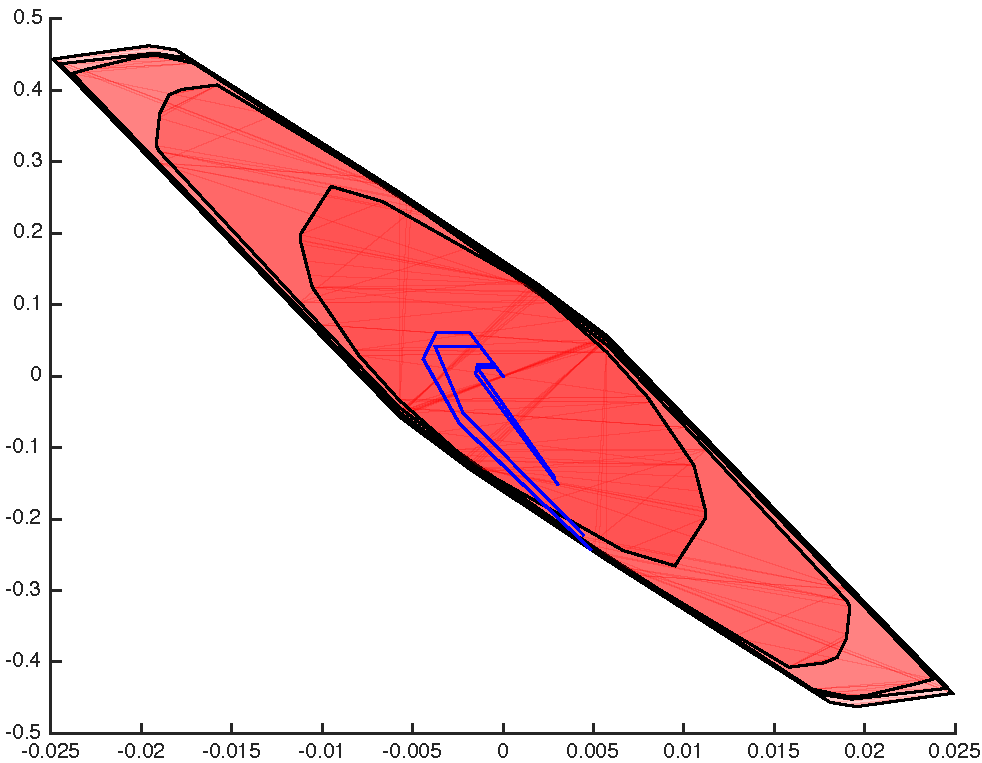
\includegraphics[width=\columnwidth]{myplot}
\caption{Projected stage constraints $\mathcal X_i, i=1,\dots,N$ in red. Trajectories
at the active set changes and on the boundary in blue.}
\label{fig:plot}
\end{figure}

% This section we present a numerical simulation in which the state-dependent uncertainty enters through an upper bound on the linearisation
% error for a nonlinear system. We consider an inverted pendulum described by $ml^2\ddot\varphi = mlg\sin\varphi+M$, where
% $m=0.1$\,kg is the mass, $l=0.3$\,m is the length of the pendulum, $g=9.81$\,m\,s$\mbox{}^{-2}$ is the gravitational
% constant and $M$ is the direct torque input. Discretisation using Euler backward finite differences 
% at $f = 20$\,Hz yields
% \begin{equation}
%   \begin{split}
%     x_1[k+1] &= x_1[k] + \frac{1}{f} x_2[k]\\
%     x_2[k+1] &= \frac{g}{fl} \sin(x_1[k]) + x_2[k] + \frac{1}{fml^2}u[k]
%   \end{split}
% \end{equation}
% where $x_1[k] = \varphi(t_0+k/f),x_2[k] = \dot\varphi(t_0+k/f)$ and $u[k] = M(t_0+k/f)$.
% The nonlinearity is given by the sine function, and we can explicitly state the 
% linearisation error as $e(x_1)=\frac{g}{fl}(\sin x_1 - x_1)$. Since the linearisation
% only approximates the nonlinear dynamics around the equilibrium we can choose a closed interval 
% $0\in D\subset\mathbb R$ and maximise the upper bound 
% \begin{equation}
%   \Delta e = \max_{x_1\in D}\abs{\frac{de}{dx_1}} = \frac{g}{fl}\max_{x_1\in D}\abs{\cos x_1-1}.
% \end{equation}
% This results in the linear system
% \begin{equation}
%   x^+ = \underbrace{\left(\begin{array}{cc}
%   1 & f^{-1}\\ g(fl)^{-1} & 1
%   \end{array}\right)}_A x + \underbrace{\left(\begin{array}{c} 0 \\(ml^2f)^{-1} \end{array}\right)}_B u
%   +\left(\begin{array}{c}w_1\\ w_2\end{array}\right)
% \end{equation}
% with $\abs{w_1}\leq w_{1,\max}$ and $\abs{w_2}\leq\max\{w_{2,\max},\Delta e \abs{x_1}\}$.
% We also introduce the input constraint $\abs{u}\leq3$\,N\,m and use the interval $D = [-\frac{3\pi}{4},
% \frac{3\pi}{4}]$ and a horizon of $N=7$ to obtain the sequence of state constraints $\mathcal X_m$
% depicted in Figure~\ref{fig:numerical:example}. The line search starting at the origin and
% exploring towards $\mathpzc x_e=(-6,50)$ produces the optimal trajectories at the active-set switches
% which are illustrated in blue. In pink a warm-started line search terminates on the boundary of the
% feasible set before reaching the (infeasible) state $\mathpzc x_e=(0,30)$.

\begin{figure}
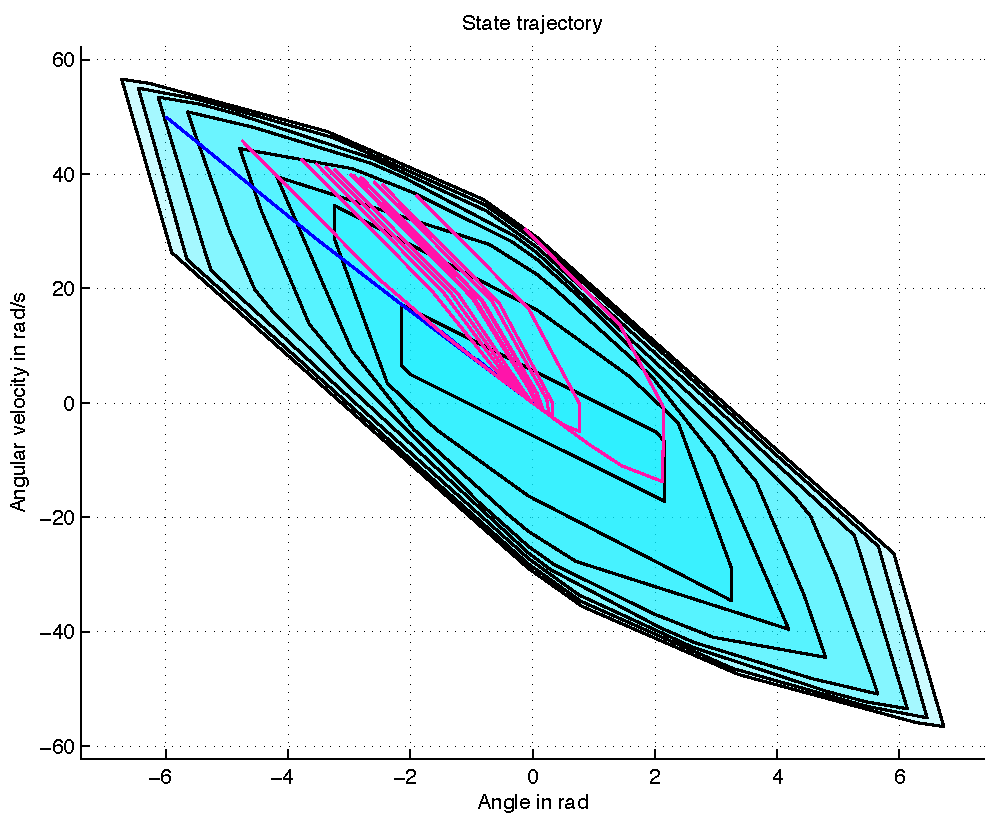
\includegraphics[width=.48\textwidth]{res}
\caption{The light blue sets depict the projected state constraint iterates~$\mathcal X_m$,
    whereas the blue and pink lines are the state trajectories produced along the two line
    searches. The pink line search eventually violates the state constraints and terminates.}
\label{fig:numerical:example}
\end{figure}
\section{Conclusion}\label{sec:conclusion}

\bibliographystyle{ifacconf}        % Include this if you use bibtex 
\bibliography{MyLib}       % and a bib file to produce the 
								                 % bibliography (preferred). The
                                 % correct style is generated by
                                 % Elsevier at the time of printing.

\end{document}
